\chapter{Data opslaan in een bestand}
Je kan data op verschillende manieren bewaren. Tekstbestanden zijn eenvoudig om te lezen, maar minder efficient om data in op te slaan. Je kan data ook binair opslaan, wat minder plaats in beslag neemt. Maar die bestanden kan je dan weer niet eenvoudig controleren met een tekst editor.

\section{Locaties}
Wat je ook kiest, je zal eerst moeten bepalen waar je data opslaat. Het is geen goed idee om zelf het hele path naar je bestand vast te leggen in code. Stel je voor dat je beslist om een config bestand op te slaan op \verb|C:\myGame\gameData\config.txt.| Dat is nogal vervelend als de gebruiker je app verplaatst naar een andere directory of schijf. De gebruiker verwacht dat de data op zijn minst in een subdirectory van je game zit. Het is zelfs mogelijk dat een computer geen C drive heeft!

Esenthel laat je toe om bepaalde paden op te vragen. Zo kan je de `documents' folder van de betreffende computer en gebruiker opvragen, zonder dat je zelf het hele path moet kennen:

\begin{code}
Str docPath = SystemPath(SP_DOCUMENTS);
\end{code}

Als je daarna een bestand wil opslaan in die `documents' folder, dan kan je het path daarvoor als volgt samenstellen:

\begin{code}
Str documentPath = S + docPath + "/myfile.txt";
\end{code} 

\begin{note}
Merk op dat je een forward slash (/) gebruikt om folders te schrijven. In Windows gebruik je normaal een backslash, maar Esenthel zal die zelf omzetten. De bedoeling is dat je met deze engine een app kan maken die ook op andere systemen --zoals Linux, mac of Android-- werkt. Andere systemen gebruiken steeds een forward slash.
\end{note}

Naast \verb|SP_DOCUMENTS| kan je nog andere systeempaden opvragen:

\begin{itemize}
\item \textbf{SP\_DESKTOP} verwijst meestal naar \verb|C:/Users/*/Desktop|.
\item \textbf{SP\_APP\_DATA} verwijst naar \verb|C:/Users/*/AppData/Roaming|. Op mobiles is het het path waar een applicatie toelating heeft om data te bewaren.
\item \textbf{SP\_APP\_DATA\_EXTERNAL} verwijst ook  naar \verb|C:/Users/*/AppData/Roaming|. Maar indien een mobile system een externe SD kaart heeft, dan zal dat path gebruikt worden.
\item \textbf{SP\_ALL\_APP\_DATA} verwijst meestal naar \verb|C:/ProgramData|
\end{itemize}

Een volledig overzicht van de mogelijkheden vind je in de header file \verb|Misc $\Rightarrow$ Misc| onder de enum declaratie `SYSTEM\_PATH'. Niet alle paden zijn beschikbaar op elk systeem. Je kan bijvoorbeeld niet naar de desktop schrijven op een mobiel platform.

\begin{exercise}
Controleer waar de bovenstaande paden op jouw computer naar verwijzen. Maak een eenvoudig testprogramma dat de resulterende string voor elk van deze paden op het scherm toont. \textsl{(Project Textfiles, ex. 01)}
\end{exercise}

\section{TextData}

De class \eeClass{TextData} laat je toe op een eenvoudige manier data als text op te slaan. Deze class is vooral voor het bewaren van config files erg handig.

\subsection{Content bewaren}
Data opslaan is eenvoudig. Voor elke variabele die je wil bewaren maak je een `node'. Je kent aan die node een waarde toe, en vervolgens sla je het bestand op.

\begin{code}
TextData data;
data.getNode("name").setValue("John Doe");
data.getNode("highscore").setValue("100");
data.save(S + SystemPath(SP_DOCUMENTS) + "/config.txt");
\end{code} 

De functie \eeFunc{getNode} zal zoeken naar de naam van de node. Indien er nog geen node bestaat met die naam, dan wordt er een nieuwe node gemaakt. De functie \eeFunc{setValue} geeft de nieuwe node een waarde.

Het bestand zal de volgende inhoud bevatten:
\begin{verbatim}
name=`John Doe`
highscore=100
\end{verbatim}

\begin{exercise}
Maak een programma met de variabelen \texttt{name}, \texttt{address}, en \texttt{age}. Geef de variabelen een default waarde en sla ze op in een bestand. Controleer of het bestand de juiste waarden bevat.
\end{exercise}

\subsection{Een bestand laden}
Een bestand laden doe je zo:

\begin{code}
TextData data;
Str docPath = SystemPath(SP_DOCUMENTS);
data.load(S + docPath + "\config.txt");
\end{code}

Indien het bestand bestaat, zal het via de bovenstaande code ingelezen worden. \textsl{(De functie \eeFunc{load} geeft ook een bool als resultaat die aangeeft of dit gelukt is. In een echte applicatie controleer je best die waarde.)}

\subsection{Content lezen}
Om de inhoud van een bestand te lezen, moet je het eerst laden. Daarna kan je je zoeken naar een bepaalde node, en de inhoud van die node toewijzen aan een variabele. Omdat het altijd mogelijk is dat een node niet bestaat, neem je twee voorzorgsmaatregelen:

\begin{enumerate}
	\item Geef je variabele een default waarde. Wanneer het niet lukt om de node te laden, blijft deze waarde gewoon behouden.
	\item Haal enkel de waarde uit een node wanneer de node bestaat. Data uit een onbestaande node halen crashed je programma.
\end{enumerate}

\begin{code}
// config values
Str name = "new player";
int highScore = 0;
int credits = 100;

TextData data;
Str docPath = SystemPath(SP_DOCUMENTS);
if(data.load(S + docPath + "/config.txt")) {
   TextNode * node;
	 
	 // try finding the name
	 node = data.findNode("name");
	 if(node) {
	    name = node.asText();
	 }
	 
	 // try finding the highscore
	 node = data.findNode("highscore");
	 if(node) {
	    highScore = node.asInt();
	 }
}
\end{code}

\begin{note}
Wanneer je een node bewaart, dan kan je er eender welk type aan toekennen met de functie \eeFunc{setValue}. Maar bij het laden van een node moet je wel een onderscheid maken naargelang het type: je gebruikt \eeFunc{asInt} voor een integer, en \eeFunc{asText} voor een string. Meer mogelijkheden vind je in de header file File $\Rightarrow$ Xml. (\eeClass{TextNode} is gebaseerd op \eeClass{TextParam}.)
\end{note}

\begin{exercise}
Pas het bestand uit de vorige oefening aan via een texteditor en laadt het terug in je programma. Toon de waarden van de variabelen op het scherm. Controleer of ze correct zijn.  \textsl{(Project Textfiles, ex. 02)}
\end{exercise}

\subsection{Een class voor een config file}
Tot slot krijg je hier nog een volledig uitgewerkt voorbeeld waarop je kan voortbouwen als je je eigen config file wil maken. De bedoeling is dat je de \verb|load()| functie uitvoert bij het starten van je programma en de \verb|save()| functie bij het afsluiten. Daartussen kan je de variabelen wijzigen via de voorziene functies. \textsl{(Project Textfiles, ex. 03)}

\begin{code}
class configFile {
private:
  Str name      = "new player";
	int highscore = 0  ;
	int credits   = 100;
	
public:
  Str getName     () { return name     ; }
	int getHighscore() { return highscore; }
	int getCredits  () { return credits  ; }
	
	void setName     (C Str & name   ) { T.name      = name   ; }
	void setHighscore(  int   score  ) { T.highscore = score  ; }
	void setCredits  (  int   credits) { T.credits   = credits; }
	
	void load() {
	  TextData data;
		if(data.load(S + SystemPath(SP_APP_DATA) + "/mygame/config.txt")) {
		  TextNode * node;
			
			if(node = data.findNode("name"     )) name      = node.asText();
			if(node = data.findNode("highscore")) highscore = node.asInt ();
			if(node = data.findNode("credits"  )) credits   = node.asInt ();
	  }
  }
	
	void save() {
	  TextData data;
		data.getNode("name"     ).setValue(name     );
		data.getNode("highscore").setValue(highscore);
		data.getNode("credits"  ).setValue(credits  );
		
		data.save(S + SystemPath(SP_APP_DATA) + "/mygame/config.txt");
  }
}
configFile ConfigFile;
\end{code}	

\section{Binary Files}
De TextData files hierboven zijn vooral handig voor configuratiebestanden of andere bestanden die je ook wil kunnen openen in een tekst editor. Ze zijn niet de meest effici\"ente manier om data op te slaan. Met de class \verb|File| kan het veel compacter. Met \verb|File| sla je enkel de waarde van een variabele op, zonder een ID om die terug te vinden:

\begin{code}
File f;                  // create file object
f.write("file.dat"    ); // start writing to a file
f.putInt(128          ); // write an integer
f.putFlt(3.14         ); // write a float
f.putStr("Hello world"); // schrijf een tekst naar het bestand
\end{code}

Wanneer je nadien de data terug wil inlezen, dan doe je dat in dezelfde volgorde. De functie \eeFunc{readTry} zorgt er voor dat de waarden enkel gelezen worden wanneer het bestand bestaat. Er bestaat ook de functie \eeFunc{read}, maar die crashed het programma wanneer een ongeldig bestand wordt gelezen.

\begin{code}
File f;
if (f.readTry("file.dat")) {
	int   i    = f.getInt();
	float pi   = f.getFlt();
	Str   text = f.getStr();
}
\end{code}

\begin{exercise}
Maak een gui class met een \eeClass{TextLine}, een \eeClass{Slider}, een \eeClass{CheckBox} en twee \eeClass{Button}'s. De eerste button bewaart de huidige waarde van de gui elementen in een bestand. De tweede button laadt dat bestand opnieuw en kent de opgeslagen waarden toe aan de gui elementen. Wijzig de gui na het opslaan en controleer of na het laden alle elementen terug de juiste waarde hebben. 
\end{exercise}

\subsection{Data Order}
Wat als je data in een andere volgorde leest en schrijft? Bekijk even de volgende code:

\begin{code}
void save() {
  File f;
	f.write("trouble.dat");
	f.putBool(true);
	f.putInt (12  );
}

void load() {
  File f;
	f.read("trouble.dat");
	int i = f.getInt ();
	int b = f.getBool();
}
\end{code}

Bij het laden en opslaan van de data werd een andere volgorde gebruikt. De compiler zal deze fout niet opmerken. Een bool variabele is precies 1 bit groot, maar een integer bestaat uit 32 bits. Er worden dus 33 bits opgeslagen: 1 + 32. Bij het laden wordt eerst de integer gelezen, maar vooraan in het bestand staat de bool variabele. Het programma laadt dus 32 bits, maar dat zijn de bool en 31 bits van de integer. Daarna wordt de laatste bit van de integer gelezen als bool. Figuur \ref{fig:filebits} illustreert dit.

\begin{figure}[ht]
\centering
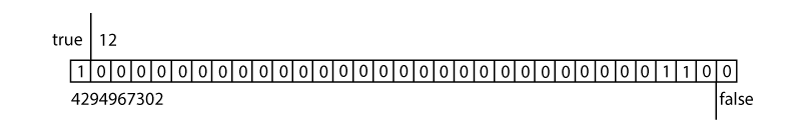
\includegraphics[width=0.8\linewidth]{../images/filebits.png}
\caption[]{bits in een bestand}
\label{fig:filebits}
\end{figure}

\begin{note}
De volgorde van de variabelen bij het lezen en het schrijven van een \verb|File| moet exact dezelfde zijn. Als je daar fouten tegen maakt, dan kan je programma crashen of zich anders gedragen dan je zou verwachten. 
\end{note}

En er is nog een andere, minder opvallende manier waarop dit mis kan gaan. C++ behandelt de argumenten van een functie van rechts naar links (net zoals de meeste andere programmeertalen, overigens). Als voorbeeld een stukje code.

\begin{code}
float r = 0.1;
float x = 0.3;
float y = 0.4;

Circle c;
c.set(r, x, y);
\end{code}

Argumenten worden gelezen van rechts naar links. Dat betekent dat de instructie \eeFunc{pos2.set} op de volgende manier wordt uitgevoerd:

\begin{enumerate}
	\item Geef de waarde van y aan het derde argument van set.
	\item Geef de waarde van x aan het tweede argument van set.
	\item Geef de waarde van r aan het eerste argument van set.
	\item Voer de functie set uit.
\end{enumerate}

Waarom is deze volgorde belangrijk? Wel, in het bovenstaande voorbeeld helemaal niet. De data die we gebruiken is niet sequentieel, ze moet niet in de juiste volgorde gelezen worden. We kunnen op elk moment de waarden van x, y of r raadplegen. Maar wat als we data uit een bestand halen? 

\begin{code}
float r = 0.1;
float x = 0.3;
float y = 0.4;

// Put data in an imaginary file
f.putFlt(r);
f.putFlt(x);
f.putFlt(y);

// ... after loading this data
Circle c;
c.set(f.getFlt(), f.getFlt(), f.getFlt());
\end{code}

De eerste float in het bestand bevat de waarde voor r. De tweede de waarde voor x en de derde voor y. Dit voorbeeld lijkt op het eerste zicht te werken, maar omdat functieargumenten van rechts naar links verwerkt worden, komt de eerste float rechts terecht. Op de plaats waar we y verwachten! Je lost dit op door er voor te zorgen dat de inhoud stap voor stap gelezen wordt. In dit geval kan dat door vooral de functie set niet te gebruiken.

\begin{code}
Circle c;
c.r     = f.getFlt();
c.pos.x = f.getFlt();
c.pos.y = f.getFlt();
\end{code}

\begin{exercise}
Maak een kort programma dat deze fout demonstreert. (Je gebruikt dus opzettelijk de foute manier.) \textsl{(Project Textfiles, ex. 04)}
\end{exercise}

\subsection{Objecten Opslaan}
Je kan ook meerdere objecten opslaan in hetzelfde bestand. Om dit te doen, geef je een \eeClass{File} object door als referentie. Zo bijvoorbeeld in de volgende class:

\begin{code}
class resource {
  int type  ;
	Vec pos   ;
	int amount;
	
	void create(int type, int amount, C Vec & pos) {
	  T.type   = type  ;
		T.pos    = pos   ;
		T.amount = amount;
	}
	
	// ... other functions are omitted to keep this example short ...
	
	void save(File & f) {
	  f.putInt(type  );
		f.putFlt(pos.x ).putFlt(pos.y).putFlt(pos.z);
		f.putInt(amount);
	}
	
	void load(File & f) {
	  type   = f.getInt();
		pos.x  = f.getFlt();
		pos.y  = f.getFlt();
		pos.z  = f.getFlt();
		amount = f.getInt();
	}
}	
\end{code}

Vervolgens voorzie je een manager class om die resources te beheren. Naast functies om ze toe te voegen, te verwijderen, op het scherm te tekenen etc., voeg je functies toe om alle bestaande resources op te slaan of te laden:

\begin{code}
class resourceManager {
  Memx<resource> resources;
	
	void save() {
		File f;
		f.write("resources.dat");
		
		f.putInt(resources.elms());
		FREPA(resources) {
			resources[i].save(f);
		}
	}
	
	void load() {
	  File f;
		if(f.readTry("resources.dat")) {
			
			int elms = f.getInt();
			for(int i = 0; i < elms; i++) {
				resources.New().load(f);
			}
		}
	}
}

resourceManager RM;
\end{code}

Je kan zelfs alle data voor je programma opslaan in hetzelfde bestand, door ook in de manager class de File als referentie door te geven in plaats van ze ter plaatse te defini\"eren. In dat geval zou je bijvoorbeeld op de volgende manier je data opslaan:

\begin{code}
void save() {
  File f;
	f.write("allData.data");
	Config.save(f);
	RM    .save(f);
}

void load() {
	File f;
	f.load("allData.data");
	Config.load(f);
	RM    .load(f);
}
\end{code}

\begin{exercise}
Maak een class voor een cirkel die ook zijn kleur kan onthouden. Voorzie een manager class die cirkels kan bevatten. Elke klik met de muis voegt een cirkel toe aan de manager, op de huidige positie van de muis en in een willekeurige kleur. (Herlees hoofdstuk \ref{section:managerClass} indien nodig.)

Zorg dat bij het afsluiten van het programma alle cirkels bewaard worden. Bij de start van het programma laadt je alle cirkels van de vorige sessie. \textsl{(Project Textfiles, ex. 05)}
\end{exercise}


